%% Generelle Dokumenteigenschaften
\documentclass[headexclude,footexclude,12pt,BCOR0pt,DIV15]{scrartcl}
\parindent0.0em
\usepackage[T1]{fontenc}
\usepackage[german]{babel}
\usepackage[latin1]{inputenc}
\usepackage{ae,aecompl}
\newcommand{\p}{\paragraph{}}  %% neuer Absatz
\newcommand{\CoMa}{\textbf{CoMa}}
\ifpdfoutput{%
  \usepackage[pdftex]{graphicx}
  \usepackage[pdftex,plainpages=false]{hyperref}
  \pdfcompresslevel=9
  \hypersetup{a4paper,pdftitle={CoMa - ein  Konferenz-Manager},pdfsubject={eine Spezifikation},pdfauthor={Sandro Esquivel, Tom Scherzer, Jan Waller},pdfborder=0}
  \DeclareGraphicsExtensions{.jpg, .pdf, .mps, .png}
}{%
  \usepackage[plainpages=false]{hyperref}
  \usepackage{graphicx}
  \DeclareGraphicsExtensions{.eps}
}

\begin{document}
%%%%%%%%%%%%%%%%%%%%%%%%%%%%%%%%%%%%%%%%%%%%%%%%%%%%%%%%%%%%%%%%%%
%%                                                              %%
%%                          Titelseite                          %%
%%                                                              %%
%%%%%%%%%%%%%%%%%%%%%%%%%%%%%%%%%%%%%%%%%%%%%%%%%%%%%%%%%%%%%%%%%%
\thispagestyle{empty}
\begin{center}
{\huge \bf \emph{CoMa - ein Konferenz-Manager}}

\vspace{2cm}

{\Large eine Spezifikation}

\vspace{2.25cm}


\includegraphics[width=5cm]{CAU-Siegel}

\vspace{2.25cm}

{\large
{\sc Christian-Albrechts-Universit\"{a}t zu Kiel} \\
Institut f\"{u}r Informatik und Praktische Mathematik \\
Lehrstuhl f\"{u}r Software-Technologie }

\vspace{2cm}

\begin{tabular}{ll}
ausgearbeitet von:           & {Sandro Esquivel} \\
                             & {Tom Scherzer} \\
                             & {Jan Waller} \\
\end{tabular}

\vspace{1cm}

Kiel, \today
\end{center}

\pagebreak
%%%%%%%%%%%%%%%%%%%%%%%%%%%%%%%%%%%%%%%%%%%%%%%%%%%%%%%%%%%%%%%%%%
%%                                                              %%
%%                     Inhaltsverzeichnis                       %%
%%                                                              %%
%%%%%%%%%%%%%%%%%%%%%%%%%%%%%%%%%%%%%%%%%%%%%%%%%%%%%%%%%%%%%%%%%%
\thispagestyle{plain} \pagenumbering{roman} \setcounter{page}{1}
\tableofcontents

\pagebreak
%%%%%%%%%%%%%%%%%%%%%%%%%%%%%%%%%%%%%%%%%%%%%%%%%%%%%%%%%%%%%%%%%%
%%                                                              %%
%%                       Text der Arbeit                        %%
%%                                                              %%
%%%%%%%%%%%%%%%%%%%%%%%%%%%%%%%%%%%%%%%%%%%%%%%%%%%%%%%%%%%%%%%%%%

\pagestyle{headings} \pagenumbering{arabic} \setcounter{page}{1}



\section{Einleitung: Motivation und Zweckbeschreibung}

    Die \emph{Vorbereitung, Organisation und Durchf\"{u}hrung einer wissenschaftlichen Konferenz},
    eines Workshops oder eines vergleichbaren Ereignisses stellt f\"{u}r die Organisatoren
    eine gro{\ss}e Herausforderung dar: \emph{Logistische Aufgaben und Probleme} sind ebenso zu
    bew\"{a}ltigen wie \emph{inhaltliche Fragen} zu kl\"{a}ren, um einen m\"{o}glichst reibungslosen Ablauf
    des Ereignisses zu erreichen und die Veranstaltung zu einem Erfolg werden zu lassen.
    \\
    \\
    Im Mittelpunkt des Interesses steht dabei der Inhalt der Konferenz, d.h. die \emph{Vortr\"{a}ge},
    die vorgestellt werden, und dementsprechend wird die meiste Konzentration auf deren
    geeignete Auswahl und Zusammenstellung verwendet. Erschwert wird dieses Prozedere
    nicht nur durch Restriktionen von au{\ss}en (z.B. kurze Dauer der Veranstaltung, Zeitmangel),
    sondern vor allem durch die komplizierten asynchronen Abl\"{a}ufe und Abh\"{a}ngigkeiten, die kaum
    vermeidbar sind, wenn mehrere (meist vielbesch\"{a}ftigte) Beteiligte, noch dazu aus aller Welt,
    koordiniert werden m\"{u}ssen.
    \\
    \\
    Doch zum Gl\"{u}ck gibt es \CoMa: ein webbasiertes Tool, welches das Auswahlverfahren der Artikel
    sinnvoll unterst\"{u}tzt, leicht zu bedienen ist und ebenso schnell wie einfach auch an speziellere
    Bed\"{u}rfnisse angepasst werden kann.
    \\
    \\
    \CoMa\ hilft bei der Zusammenstellung des \emph{Komitees}, bei der \emph{Einladung der Autoren}, die
    \"{u}ber ihr eigenes Nutzerprofil selbst\"{a}ndig \emph{Artikel} online einreichen k\"{o}nnen, und vor
    allem bei der effizienten \emph{Auswahl der besten Artikel}. Selbstverst\"{a}ndlich werden Nutzerdaten,
    Beitr\"{a}ge, Artikel, Diskussionen, Entscheidungen und Bewertungen der Beteiligten nur dem
    jeweils daf\"{u}r vorgesehenen Personenkreis zug\"{a}nglich gemacht, um ein hohes Ma{\ss} an \emph{Diskretion}
    auch unter den Teilnehmern selbst sicherzustellen.

    Vor allem aber etabliert \CoMa\ einen Standard f\"{u}r die \emph{Kommunikation} aller Beteiligten
    untereinander - und ist als Webanwendung f\"{u}r jeden sofort ohne Installationsaufwand
    und von \"{u}berall aus nutzbar.

    \pagebreak

\section{Spezifikation der Benutzer und Objekte}

    \begin{center}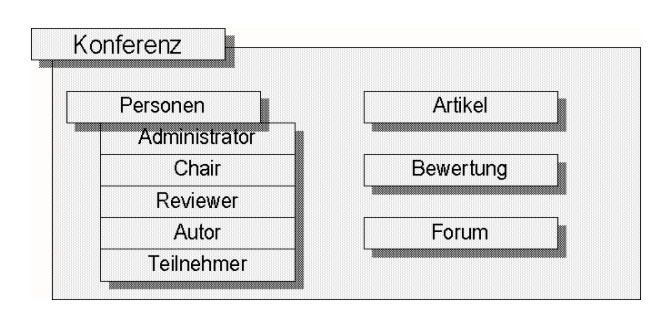
\includegraphics[width=17cm]{uebersicht1}\end{center}

    \subsection{Allgemeine Rollenverteilung}

       Eine \emph{Person} ist im folgenden ein Benutzer in \CoMa, dem ein Account
       zugeordnet ist. Interaktionen und Benachrichtigungen findet \"{u}ber diese Accounts statt.
       Jeder Person k\"{o}nnen mehrere \emph{Rollen} zugeteilt sein, wobei \"{u}ber den Account je eine
       Rolle zur Zeit \"{u}bernommen werden kann. \CoMa\ unterscheidet zwischen folgenden Rollen:

        \begin{description}
            \item[Administrator:] Der Administrator ist f\"{u}r die Installation von \CoMa\ und f\"{u}r
                die Behebung etwaiger Probleme w\"{a}hrend des Betriebs verantwortlich.

            \item[Chair:] Ein (gleichberechtigter) Vorsitzender des Programmkomitees, das aus (mindestens)
                einem Chair und mehreren Reviewern besteht und f\"{u}r die Einladung/Wahl der Autoren und die
                Auswahl der besten Artikel verantwortlich ist.

            \item[Reviewer:] Ein Mitglied des Programmkomitees auf Einladung eines Chairs, beteiligt sich
                an der Diskussion und Bewertung von bestimmten, ihm zugewiesenen Artikeln.

            \item[Autor:] Ein Autor bewirbt sich oder wird (selten) von den Chairs eingeladen, Artikel einzureichen,
                die er bei Annahme auf der Konferenz vorstellt.

            \item[Teilnehmer:] Ein Teilnehmer an der Konferenz hat nur Zugriff auf einige \"{o}ffentliche Informationen
                und Funktionalit\"{a}ten.

        \end{description}

        Als \emph{Co-Autoren} bezeichnen wir im folgenden solche Personen, die als Co-Autor eines Artikels
        gelistet oder anderweitig befangen sind, und daher nicht an der Bewertung eines Artikel teilhaben d\"{u}rfen.
        Co-Autoren werden nicht durch eine eigene Rolle repr\"{a}sentiert.

    \subsection{Allgemeine Begriffe und Objekte}

        Als \emph{Objekte} in \CoMa\ bezeichnen wir im folgenden Personen und diese Begriffe:

        \begin{description}
            \item[Artikel:] Ein Dokument, welches ein Autor einreicht, um es auf der Konferenz
                vorzustellen. Wird von Reviewern bewertet.

            \item[Bewertung:] Eine notenbasierte Bewertung in verschiedenen Kategorien, die durch die Reviewer
                entschieden und eventuell revidiert wird. Artikel werden nach ihrer Gesamtbewertung
                linear sortiert. Dienen als Hilfe bei der Entscheidung, Artikel anzunehmen oder abzulehnen.

            \item[Forum:] Eine threadbasierte Mitteilungsplattform, die je nach Art des Forums f\"{u}r
                          verschiedene Teilnehmer zug\"{a}nglich ist (\"{o}ffentliches Forum f\"{u}r alle Benutzer,
                          Komiteeforum f\"{u}r Chairs und Reviewer, Artikelforum f\"{u}r Komitee bis auf
                          die Autoren des Artikels).

            \item[Konferenz:] Die Menge aller Benutzer, Dokumente und Konferenzdaten einer Konferenzinstanz.
                              \CoMa\ kann mehrere Konferenzinstanzen parallel verwalten.

        \end{description}

    \subsection{Charakterisierung aller Objekte}

        \subsubsection{Person}
        \begin{itemize}
            \item Pers\"{o}nliche Daten (Name, Anschrift, e-Mail, Beschreibung, Benutzername,
                  Passwort) und Optionen zum \texttt{[\"{A}ndern]} und \texttt{[Zur\"{u}cksetzen]} der Daten
            \item Zugang zum \"{o}ffentlichen Forum
            \item Pers\"{o}nliche $\rightarrow$Systemnachrichten
            \item Liste aller $\rightarrow$Rollen und entsprechende Anzeigen/Interaktionsm\"{o}glichkeiten
        \end{itemize}

        \subsubsection{Autor}
        \begin{itemize}
            \item Liste seiner eingereichten $\rightarrow$Artikel mit den Optionen \texttt{[Hinzuf\"{u}gen]},
                  \texttt{[Aktualisieren]}, \texttt{[Entfernen]}
            \item Status seiner Artikel (wenn diese entschieden sind)
            \item Option zum \texttt{Zur\"{u}ckziehen} seines Accounts
        \end{itemize}

        \pagebreak

        \subsubsection{Reviewer}
        \begin{itemize}
            \item Bevorzugte Themen (m\"{u}ssen zum Beginn der Reviewphase verbindlich gew\"{a}hlt sein)
            \item W\"{a}hrend der Auswahlphase: Liste aller bisher eingegangenen Artikel mit Option zum Markieren als
                  \texttt{[Gew\"{u}nscht]}, \texttt{[Keine Angabe]}, \texttt{[Nicht gew\"{u}nscht]} und \texttt{[ist Co-Autor von]}.
            \item Liste der ihm zugeteilten $\rightarrow$Artikel
            \begin{itemize}
                \item Eigenes $\rightarrow$Bewertungsformular (solange der Artikel nicht entschieden ist, bis zur Deadline des Artikels)
                \item Status des Artikels (entschieden/nicht entschieden, Anzahl der abgegebenen Bewertungen; wird diskutiert,
                    aktuelle durchschnittliche Bewertung, wenn er seine Bewertung abgegeben hat)
                \item Zugang zur Artikeldiskussion (wenn er seine Bewertung abgegeben hat)
                \item Deadline f\"{u}r den Artikel
                \item Option zum \texttt{[Ablehnen]} der Artikelbewertung
            \end{itemize}
            \item Liste aller bereits bewerteten $\rightarrow$Artikel (die ihm nicht zugeteilt sind und von denen er nicht (Co-)Autor ist)
            \begin{itemize}
                \item Status des Artikels (s.o.)
                \item Zugang zur Artikeldiskussion (wobei er als nicht zur Reviewergruppe geh\"{o}rig
                gekennzeichnet wird)
            \end{itemize}
            \item Option zum \texttt{[Zur\"{u}ckziehen]} seines Accounts
        \end{itemize}

        \subsubsection{Teilnehmer}
        \begin{itemize}
            \item zus. Teilnehmerdaten (z.B. Tarif, Zahlungsmethode, besondere Pr\"{a}ferenzen)
                  $\longrightarrow$ wird in dieser Spezifikation im folgenden noch nicht ber\"{u}cksichtigt
            \item Option zum \texttt{[Zur\"{u}ckziehen]} seiner Teilnahme
        \end{itemize}

        \subsubsection{Chair}
        \begin{itemize}
            \item $\rightarrow$\texttt{[Konfiguration]} der Konferenz
            \item Benutzerverwaltung
            \begin{itemize}
                \item Chairs, Reviewer, Autoren und Teilnehmer \texttt{[einladen]}
                \item Liste aller bestehenden Accounts (Name und Rollen) mit den Optionen
                    \texttt{[Entfernen]}, \texttt{[Rolle hinzuf\"{u}gen/entfernen]}, \texttt{[Benachrichtigen]}
            \end{itemize}
            \item Artikelverwaltung
            \begin{itemize}
                \item Liste aller eingesandten $\rightarrow$Artikel (Autor, Titel, Beschreibung, Status, Bewertungen, Diskussion)
                    mit den Optionen \texttt{[Ansehen]}, \texttt{[L\"{o}schen]}, \texttt{[Kommentar f\"{u}r Chairs hinzuf\"{u}gen]}
            \end{itemize}
            \item Verteilung (Teil der Artikelverwaltung)
            \begin{itemize}
                \item Liste der Artikel wie oben mit den Optionen \texttt{[Reviewer hinzuf\"{u}gen]}, \texttt{[Reviewer verbieten]},
                    \texttt{[Reviewerliste]}, Status (unverteilt/weitere Reviewer n\"{o}tig)
                \item Namen der Reviewer mit den Optionen \texttt{[Reviewer entziehen]}, \texttt{[Reviewer hinzuf\"{u}gen]}, \texttt{[Benachrichtigen]}
                \item Option \texttt{[Verteilung vorschlagen lassen]}, \texttt{[Verteilung \"{u}bernehmen]}, \texttt{[Reviewphase starten]}
            \end{itemize}
            \item Entscheidung (Teil der Artikelverwaltung)
            \begin{itemize}
                \item Liste der Artikel wie oben mit den Optionen \texttt{[Annehmen]}, \texttt{[Ablehnen]}
                \item \texttt{[Beenden]} der Entscheidungsphase
            \end{itemize}
        \end{itemize}

        \subsubsection{Bewertungsformular}
        \begin{itemize}
            \item Liste der Bewertungskriterien (auch: Gesamtbewertung)
            \begin{itemize}
                \item Bewertungskommentarfeld
                \item Bewertung (im festgelegten Notenspektrum, auch: Enthaltung)
            \end{itemize}
            \item \texttt{[Abschicken]}/\texttt{[Aktualisieren]} der Bewertung
        \end{itemize}

        \subsubsection{Artikel}
        \begin{itemize}
            \item Artikeldaten (Titel, Beschreibung, Autor, Co-Autoren, Erstellungsdatum, \"{A}nderungsdatum, Versionsnummer)
            \item Artikelthemen (aus der Liste der vorgegebenen Themen)
            \item Datei (Bin\"{a}rdaten und MIME-Type) und Optionen zum \texttt{[Herunterladen]} und \texttt{[Ansehen]}
            \item Bewertung und Status
            \begin{itemize}
                \item Liste der Reviewer und deren (Gesamt-)Bewertungen
                \item Gesamtbewertung
                \item Status (Angenommen, abgelehnt, nicht eindeutig bewertet, Bewertung abgeschlossen)
            \end{itemize}
        \end{itemize}

\pagebreak

        \subsubsection{Konfiguration der Konferenz}
        \begin{itemize}
            \item Initiale Konfiguration
            \begin{itemize}
                \item Vollst\"{a}ndige Liste der m\"{o}glichen Artikelthemen
                \item Erweiterte Konfiguration:
                \begin{itemize}
                    \item Liste der Bewertungskriterien (verschiedene Schemata)
                    \item Notenspektrum (Standard: \textit{1-5})
                \end{itemize}
                \item Option zum \texttt{[Einrichten]} der Konferenz mit den initialen Einstellungen
            \end{itemize}
            \item Allgemeine Konfiguration
            \begin{itemize}
                \item W\"{a}hrend aller Phasen m\"{o}glich
                \item Deadlines (Beginn der Reviewphase, Ende der Reviewphase; nur vor Ablauf der Deadline \"{a}nderbar)
                \item Konferenzdaten (Titel, Beschreibung, Ort, Zeit, Homepage)
                \item Anzahl der anzunehmenden Artikel (min/max)
                \item Erweiterte Konfiguration:
                \begin{itemize}
                    \item Anzahl der Reviewer pro Artikel (min/gew\"{u}nscht) (Standard: \textit{3/4})
                    \item Als kritisch geltende Varianz der Artikelbewertungen (Standard: muss noch ermittelt werden)
                    \item Automatische Accountfreischaltung (Standard: \textit{ja})
                    \item Automatische Diskussionser\"{o}ffnung bei uneindeutigen Bewertungen (Standard: \textit{ja})
                    \item Automatische Zuteilung von zus\"{a}tzlichen Reviewern (Standard: \textit{nein})
                    \item Anzahl der zus\"{a}tzlichen Reviewer (Standard: \textit{2})
                \end{itemize}
                \item Optionen zum \texttt{[\"{U}bernehmen]} und \texttt{[Zur\"{u}cksetzen]} der Einstellungen
            \end{itemize}
        \end{itemize}

        \subsubsection{Forum}
        \begin{itemize}
            \item Forendaten (Titel, Beschreibung)
            \item Sichtbarkeit des Forums (\"{o}ffentlich, nur f\"{u}r Komitee, Artikelforum)
            \item Bei Artikelforen: zugeordneter Artikel
            \item Liste der Threads (Thema, Ersteller, Erstellzeit)
            \begin{itemize}
                \item Liste der Postings (Ersteller, Erstellzeit, Text)
                \item Optionen \texttt{[Antworten]}/\texttt{[Posting l\"{o}schen]} (nur Chair)
            \end{itemize}
            \item Optionen \texttt{[Neuen Thread erstellen]}/\texttt{[Thread lesen]}
        \end{itemize}

\pagebreak

    \subsection{Das Datenmodell f\"{u}r die Konferenz}
\begin{center}
    \begin{tabular}{|c|}
      \hline
      \emph{Conference} \\
      \hline
      \underline{id} \\
      title \\
      description \\
      location, time \\
      homepage \\
      \textbf{configuration:} \\
      submitPaperDeadline \\
      submitReviewDeadline \\
      minPapers, maxPapers \\
      \textbf{extended configuration:} \\
      topicNames* (\textit{common topics}) \\
      ratingCriteria* (\textit{common criteria}) \\
      ratingType (\textit{1: 1-5}) \\
      minReviewersPerPaper (\textit{3}) \\
      averageReviewersPerPaper (\textit{4}) \\
      criticalVariance (\textit{?$\cdot\sigma$}) \\
      autoValidateAccounts? (\textit{true}) \\
      autoStartPaperDiscussion? (\textit{true}) \\
      autoAddRereviewers? (\textit{false}) \\
      numRereviewers (\textit{2}) \\
      \hline
    \end{tabular}
    \begin{tabular}{|c|}
      \hline
      \emph{Person} \\
      \hline
      \underline{id} \\
      name \\
      address \\
      email \\
      phone \\
      description \\
      username \\
      password \\
      deleted? \\
      \hline
    \end{tabular}
    \begin{tabular}{c}
      \begin{tabular}{|c|}
        \hline
        \emph{Chair ($\rightarrow$ Person)} \\
        \hline
        \textit{none} \\
        \hline
      \end{tabular} \\
      \\
      \begin{tabular}{|c|}
        \hline
        \emph{Reviewer ($\rightarrow$ Person)} \\
        \hline
        $\longrightarrow$ papers* \\
        $\longrightarrow$ reviews* \\
        $\longrightarrow$ preferredTopics* \\
        \hline
      \end{tabular} \\
      \\
      \begin{tabular}{|c|}
        \hline
        \emph{Author ($\rightarrow$ Person)} \\
        \hline
        $\longrightarrow$ papers* \\
        \hline
      \end{tabular} \\
      \\
      \begin{tabular}{|c|}
        \hline
        \emph{Participant ($\rightarrow$ Person)} \\
        \hline
        \textit{none} \\
        \hline
      \end{tabular} \\
    \end{tabular} \\

    \begin{tabular}{|c|}
      \hline
      \emph{Paper} \\
      \hline
      \underline{id} \\
      title \\
      abstract \\
      createDate, editDate \\
      version \\
      $\longrightarrow$ author \\
      coauthors* \\
      $\longrightarrow$ topics* \\
      mimeType \\
      data \\
      \hline
    \end{tabular}
    \begin{tabular}{|c|}
      \hline
      \emph{ReviewedPaper ($\rightarrow$ Paper)} \\
      \hline
      $\longrightarrow$ reviewers[] \\
      ratings* \\
      totalRating \\
      accepted? \\
      reviewed? \\
      decided? \\
      critical? \\
      \hline
    \end{tabular}
    \begin{tabular}{|c|}
      \hline
      \emph{Review} \\
      \hline
      $\longrightarrow$ reviewer \\
      $\longrightarrow$ paper \\
      ratings* \\
      comments* \\
      totalRating \\
      \hline
    \end{tabular}

    \begin{tabular}{|c|}
      \hline
      \emph{Message} \\
      \hline
      \underline{id} \\
      $\longrightarrow$ receiver \\
      sendTime \\
      priority \\
      text \\
      read? \\
      \hline
    \end{tabular}
    \begin{tabular}{|c|}
      \hline
      \emph{Forum} \\
      \hline
      \underline{id} \\
      title \\
      description \\
      $\longrightarrow$ threads* \\
      visibility \\
      $\longrightarrow$ paper \\
      \hline
    \end{tabular}
    \begin{tabular}{|c|}
      \hline
      \emph{Thread} \\
      \hline
      \underline{id} \\
      title \\
      $\longrightarrow$ creator \\
      createTime \\
      $\longrightarrow$ postings* \\
      \hline
    \end{tabular}
    \begin{tabular}{|c|}
      \hline
      \emph{Posting} \\
      \hline
      \underline{id} \\
      $\longrightarrow$ creator \\
      createTime \\
      text \\
      $\longrightarrow$ nextPosting \\
      \hline
    \end{tabular}
\end{center}
\pagebreak
        Anmerkungen zum Datenmodell:
        \begin{itemize}
            \item \texttt{id} ist eindeutig und wird automatisch vom System vergeben.
            \item \texttt{password} wird codiert gespeichert.
            \item Versionsnummern werden bei Updates automatisch hochgez\"{a}hlt.
            \item * kennzeichnet Felder (bzw. $1$:$n$-Beziehungen).
            \item ? kennzeichnet \texttt{boolean}-Werte (\textit{ja}/\textit{nein}).
            \item Standardwerte sind in nachgestellten Klammern vermerkt.
        \end{itemize}

    \subsection{ER-Diagramm f\"{u}r das Datenmodell}
        \begin{center}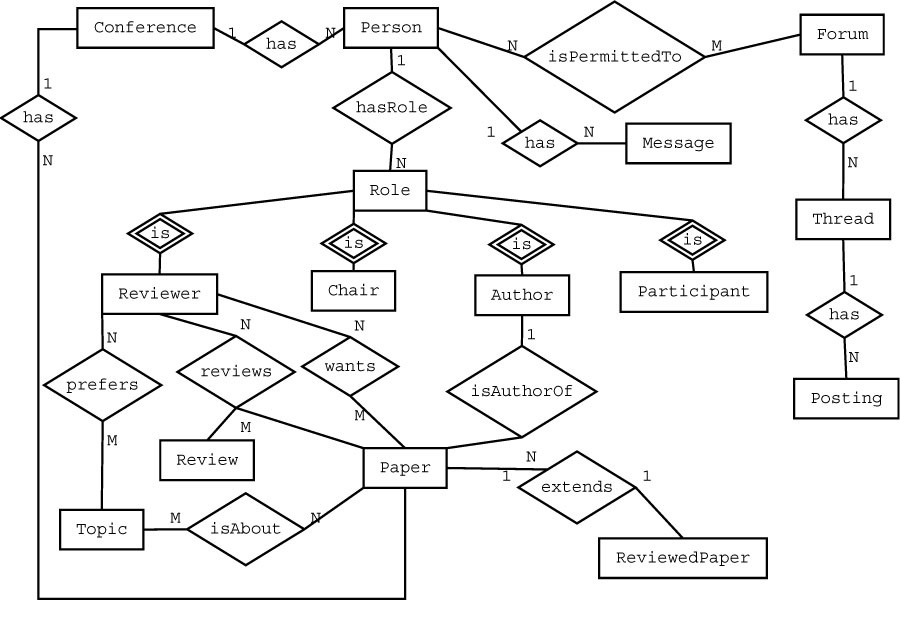
\includegraphics[width=15cm]{CoMa-ER-Diagramm}\end{center}
        W\"{a}hrend das vorangegangene Kapitel das Datenmodell anhand der Objekte und ihrer Attribute
        beschreibt, soll das ER-Diagramm die Beziehungen zwischen den Objekten, insbesondere deren
        Kardinalit\"{a}ten verdeutlichen. \\
        Es fehlt hier die $n$:$m$-Beziehung 'isCoAuthorOf' zwischen Artikeln und Co-Autoren.
        N\"{a}here Erl\"{a}uterungen dazu sind in $\rightarrow$\ref{CoAutoren} zu finden.

\pagebreak

    \section{Spezifikation der Abl\"{a}ufe und Interaktionen}
    \begin{center}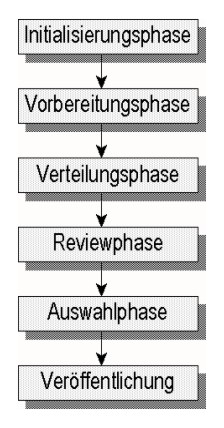
\includegraphics[width=4cm]{ablauf1}\end{center}

    \subsection{Beschreibung der Phasen}
        Der von \CoMa\ unterst\"{u}tzte Ablauf nach der Installation und Einrichtung eines Chair-Accounts ist
        folgender (vgl. \"{U}bersicht \"{u}ber die Interaktionen):

        \subsubsection{Initialisierungsphase}
        \begin{itemize}
            \item Einstellen der gew\"{u}nschten Optionen oder \"{U}bernahme der Standard-Einstellungen
            \item einige Einstellungen sind verbindlich und nachtr\"{a}glich nicht mehr \"{a}nderbar (vollst\"{a}ndige
                Auflistung der m\"{o}glichen Themenbereiche, Bewertungskriterien)!
        \end{itemize}

        \subsubsection{Vorbereitungsphase}
        \begin{itemize}
            \item Vorbereitung, Komiteebildung, Aufnahme der Autoren und Artikel:
            \item Hinzuf\"{u}gen von weiteren Chair-Accounts.
            \item Einladung von Reviewern und evtl. Autoren durch die Chairs.
            \item Eingeladene Reviewer k\"{o}nnen einen Reviewer-Account freischalten und m\"{u}ssen gewisse
                  verbindliche Einstellungen vornehmen, bevor sie in Diskussionen/Bewertungen miteinbezogen
                  werden.
            \item Alle interessierten Autoren k\"{o}nnen einen Autoren-Account freischalten.
            \item Eventuell Pr\"{u}fung der freizuschaltenden Accounts durch den Chair.
            \item Autoren k\"{o}nnen bis zu einer vom Chair vorgegebenen (\"{a}nderbaren!) Deadline einen oder mehrere
                  Artikel einsenden, aktualisieren und auch entfernen.
            \item Reviewer k\"{o}nnen die Liste aller Artikel einsehen, gew\"{u}nschte/unerw\"{u}nschte Artikel und
                  bevorzugte Themen markieren und Artikel markieren, von welchen sie Co-Autoren sind.
        \end{itemize}

        \subsubsection{Verteilungsphase}
        \begin{itemize}
            \item Verteilung der Artikel auf Reviewer:
            \item Zun\"{a}chst treffen die Chairs eine Vorauswahl, welche Artikel von welchen Reviewern bewertet
                werden sollen bzw. nicht bewertet werden d\"{u}rfen.
            \item Verteilungsalgorithmus macht auf Grundlage der Einstellungen einen Vorschlag f\"{u}r eine Zuordnung
                von Artikeln zu Reviewern. Ber\"{u}cksichtigt werden bevorzugte Themen und Artikelw\"{u}nsche der Reviewer.
            \item Chairs k\"{o}nnen sich im Einzelfall f\"{u}r einen Artikel andere m\"{o}gliche Reviewer anzeigen lassen und ggf.
                manuelle \"{A}nderungen an dem Vorschlag vornehmen.
        \end{itemize}

        \subsubsection{Reviewphase} \label{Reviewphase}
        \begin{itemize}
            \item Review und Diskussion der Artikel (bis zur zweiten Deadline):
            \item Reviewer bewerten die ihnen zugeordneten Artikel, d.h. benoten sie in den festgelegten Kriterien
                  und schreiben einen Kommentar dazu.
            \item Reviewer k\"{o}nnen die Benotung und Kommentare jederzeit \"{a}ndern.
            \item Falls keine einheitliche Meinung gefunden wird, wird eine interne Diskussion der beteiligten
                  Reviewer (eventuell manuell durch den Chair) gestartet, die f\"{u}r weitere Reviewer desselben
                  Artikels einsehbar wird, sobald sie eine eigene Bewertung abgegeben haben. Fremde Reviewer k\"{o}nnen
                  jederzeit teilnehmen, sobald der Artikel das erste Mal bewertet wurde.
            \item Solche nicht eindeutig bewerteten Artikel werden den Chairs als kritische Artikel gemeldet.
                  Diese k\"{o}nnen dem Artikel dann weitere Reviewer (Re-Reviewer) zuordnen und Vorschl\"{a}ge f\"{u}r
                  eine Zuordnung durch \CoMa\ anzeigen lassen (vgl. Verteilung der Artikel auf Reviewer, eingeschr\"{a}nkt
                  auf die kritischen Artikel). Dieser Schritt kann automatisiert werden.
            \item Chairs k\"{o}nnen sich jederzeit \"{u}ber den Zwischenstand der Bewertung informieren, verschiedene
                  Sortierungskriterien m\"{o}glich (etwa nach einzelnen Bewertungskriterien,
                  Gesamtbewertung).
            \item Chairs k\"{o}nnen die Reviewphase eines Artikel manuell beenden.
            \item Reviewer k\"{o}nnen jederzeit Artikel ablehnen oder ihre Teilnahme beenden. Die freigewordenen
                  Artikel m\"{u}ssen durch die Chairs neu verteilt werden.
        \end{itemize}

        \pagebreak

        \subsubsection{Auswahlphase}
        \begin{itemize}
            \item Chairs w\"{a}hlen (unter Zuhilfenahme verschiedener Sortierungskriterien f\"{u}r eine \"{U}bersicht der
                  Bewertungen) Artikel aus (Markierung als angenommen/abgelehnt).
            \item Reviewer k\"{o}nnen den Status einen entschiedenen Artikels (angenommen/abgelehnt)
                  einsehen.
            \item Automatische Benachrichtigung der Autoren \"{u}ber das Ergebnis der Auswahl mit Feedback (einzelne
                  Bewertungen/Noten, Kommentare, die Reviewer bleiben aber anonym).
        \end{itemize}

        \subsubsection{Ver\"{o}ffentlichungsphase}
        \begin{itemize}
            \item Liste der ausgew\"{a}hlten Artikel wird \"{o}ffentlich zug\"{a}nglich gemacht.
            \item Automatisches Er\"{o}ffnen eines entsprechenden Threads im Forum.
            \item Es k\"{o}nnen sich nur noch Teilnehmer f\"{u}r die Konferenz anmelden.
        \end{itemize}

    \subsection{\"{U}bersichtstabelle \"{u}ber die Meldungen}

    \begin{tabular}{|c|c|c|}
      \hline
      \textbf{Ereignis} & \textbf{Empf\"{a}nger} & \textbf{Art} \\
      \hline
      \hline
      Person y wurde eingeladen. & Person y & e-Mail \\
      \hline
      Account von Person y wurde freigeschaltet. & Person y & e-Mail \\
      \hline
      Person y hat sich l\"{a}nger nicht eingeloggt. & Person y & e-Mail \\
      \hline
      Artikeleinsendung endet bald. & Autor & intern \\
      \hline
      Artikeleinsendung ist beendet. & Autor, Reviewer & intern \\
      \hline
      Artikel sind verteilt, Reviewphase beginnt. & Reviewer & intern \\
      \hline
      Es wurden Artikel an einen potentiellen & Reviewer & intern \\
      Co-Autor verteilt. & & \\
      \hline
      Reviewphase endet bald. & Reviewer & intern \\
      \hline
      Reviewphase endet bald und & Reviewer von Artikel x & intern \\
      Artikel x ist noch unbewertet. & & (e-Mail) \\
      \hline
      Artikel x ist nicht eindeutig. & Chair & intern \\
      \hline
      Diskussion zu Artikel x hat begonnen. & Reviewer von Artikel x & intern \\
      \hline
      Review von Artikel x wurde beendet. & Reviewer von Artikel x & intern \\
      \hline
      Reviewphase ist beendet. & Reviewer & intern \\
      \hline
      Artikel x wurde angenommen/nicht angenommen. & Autor/Reviewer von Artikel x & intern \\
      (f\"{u}r Autoren zus\"{a}tzlich Bewertungsdetails) & & e-Mail \\
      \hline
      Konferenzprogramm, Zeit und Ort stehen fest. & Autor, Reviewer, Teilnehmer & intern \\
       & & e-Mail \\
      \hline
    \end{tabular}

    \pagebreak

    \subsection{\"{U}bersichtstabelle \"{u}ber die Interaktionen}
        \begin{tabular}{|c|c|c|}
          \hline
          \textbf{Interaktion} & \textbf{Rollen} & \textbf{Einschr\"{a}nkung} \\
          \hline
          \hline
          Rollen hinzuf\"{u}gen/entfernen & Chair & - \\
          \hline
          Benutzer l\"{o}schen & Chair & Chair kann nicht sich selbst l\"{o}schen \\
          \hline
          Account registrieren & alle & Chairs und Reviewer m\"{u}ssen eingeladen werden, \\
          & & Teilnehmer erst nach Anmeldungsfreigabe \\
          \hline
          Account freischalten & Chair & kann automatisiert werden \\
          \hline
          Eigenen Account l\"{o}schen & alle & min. ein Chair muss existieren \\
          \hline
          Accountdaten \"{a}ndern & Chair & - \\
          \hline
          Eigene Accountdaten \"{a}ndern & alle & - \\
          \hline
          Accountdaten sehen & alle & Chair sieht alle Daten, \\
           & & andere nur \"{o}ffentliche Daten \\
          \hline
          Artikel einsenden & Autor & vor Ablauf der Einsendefrist \\
          \hline
          Artikel \"{a}ndern & Chair, & Autor nur eigene Artikel \\
           & Autor & \\
          \hline
          Artikel l\"{o}schen & Chair, & Autor nur eigene Artikel \\
           & Autor & \\
          \hline
          Artikelpr\"{a}ferenzen angeben & Reviewer & vor Beginn der Reviewphase \\
          \hline
          Artikel verteilen & Chair & nach Ablauf der Einsendefrist, \\
           & & vor Ablauf der Bewertungsfrist \\
          \hline
          zus. Reviewer verteilen & Chair & s.o., kann automatisiert werden \\
          \hline
          Verteilung vorschlagen lassen & Chair & nach Ablauf der Einsendefrist, \\
           & & vor Ablauf der Bewertungsfrist \\
          \hline
          Artikelbewertung ablehnen & Reviewer & nach Beginn der Reviewphase \\
          \hline
          Artikel sehen & alle & - \\
          \hline
          Artikelbewertungen & alle & (Co-)Autoren nicht eigene Artikel, \\
          und -status sehen & & Reviewer erst nach Abgabe eigener Bewertung \\
          \hline
          Reviewergruppe sehen & Chair, & Reviewer erst nach eigener Bewertung \\
           & Reviewer & \\
          \hline
          Artikel diskutieren & alle & (Co-)Autoren nicht eigene Artikel, \\
           & & Reviewer erst nach Abgabe eigener Bewertung \\
          \hline
          Artikel bewerten & Reviewer & nur zugeteilte Artikel, nach Beginn \\
           & & der Reviewphase, vor Ablauf der \\
           & & Bewertungsfrist oder Sperren des Artikels \\
          \hline
          Artikeldiskussion starten & Chair, & s.o., Reviewer nur f\"{u}r zugeteilte Artikel \\
           & Reviewer & \\
          \hline
          Artikelbewertung sperren, & Chair & nach Beginn der Reviewphase, \\
           Bewertungssperre aufheben & & vor Ablauf der Bewertungsfrist \\
          \hline
          Artikel annehmen/ablehnen & Chair & nach Sperren des Artikel \\
           & & oder Ablauf der Bewertungsfrist \\
          \hline
          Programm ver\"{o}ffentlichen & Chair & nach Auswahl der Artikel \\
          \hline
          Teilnehmeranmeldung freigeben & Chair & - \\
          \hline
        \end{tabular}

    \pagebreak

\section{Spezifikation von Details und Algorithmen:}

    \subsection{Anmeldesystem}
    \begin{center}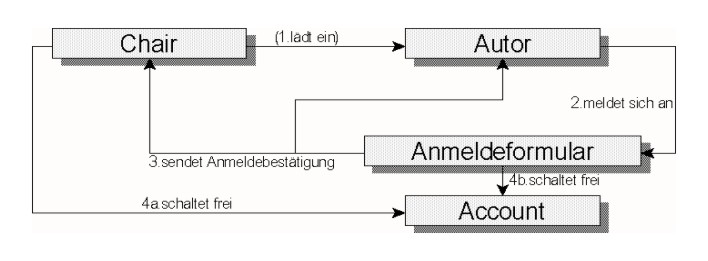
\includegraphics[width=17cm]{anmelde1}\end{center}
    Die Anmeldung von Autoren erfolgt nach folgendem Schema:\\
    Eventuell l\"{a}dt der \emph{Chair} die entsprechende Person per Formular in \CoMa\ ein. In der Regel
    meldet sich der Autor allerdings auf Eigeninitiative \"{u}ber ein \"{o}ffentlich zug\"{a}ngliches \emph{Anmeldeformular} an.
    \\
    Das \emph{Anmeldeformular} sendet dann eine Anmeldebest\"{a}tigung sowohl an den zuk\"{u}nftigen Autor, als auch
    an den Chair.\\
    Der \emph{Account} wird dann je nach Systemkonfiguration entweder automatisch oder nur nach Best\"{a}tigung der Chairs
    freigeschaltet.\\
    \\
    Die Anmeldung von weiteren Chairs oder Reviewern erfolgt dabei auf die gleiche Weise, nur das der Schritt der Einladung
    hier immer erforderlich ist. Reviewer und Chairs erhalten mit der Einladung die Zugangsdaten zu einer gesch\"{u}tzten
    \emph{Anmeldeseite}. \\

    \subsection{Konfiguration, Parameter und optionale Features} \label{Konfiguration}
      \subsubsection{Allgemeine Einstellungen}
        Die hier eingestellten Daten haben keinen gro{\ss}en Einfluss auf die Funktionen von \CoMa, sondern
        sind rein informell, und zur Darstellung von z.B. korrekten Titeln in Fenstern etc gedacht, sowie f\"{u}r eine
        eventuelle sp\"{a}tere Ver\"{o}ffentlichung des Konferenzprogrammes.\\
        \\
        \textbf{title}: Dieses Feld nimmt den Titel auf, unter dem die Konferenz l\"{a}uft.
        \\
        \textbf{description}: Hier ist Platz f\"{u}r eine kurze Beschreibung des geplanten Inhalts, der Zielgruppe etc.
        \\
        \textbf{location}: Der Ort, an dem die Konferenz stattfindet, kann hier genannt werden.
        \\
        \textbf{time}: Der Zeitpunkt, zu dem die Konferenz beginnt.
        \\
        \textbf{homepage}: Ein Verweis auf die offizielle Homepage der Konferenz (auf der \CoMa\ normalerweise auch zu finden sein sollte!).

      \subsubsection{Konfiguration}
        \textbf{submitPaperDeadline}: Hier wird die erste \emph{Deadline} von \CoMa\ eingestellt, i.e. der Zeitpunkt, zu dem keine
            weiteren Artikel mehr eingesandt werden k\"{o}nnen. Diese Einstellung kann vom \emph{Chair} jederzeit ver\"{a}ndert werden, solange die
            Deadline noch nicht abgelaufen ist, wobei eine Verschiebung in die Vergangenheit ein sofortiges Ende der Vorbereitungsphase bedeutet.
        \\
        \\
        \textbf{submitReviewDeadline}: Dieses ist die zweite wichtige \emph{Deadline}, die sich in \CoMa\ einstellen l\"{a}sst. Das Ende dieser
            Deadline l\"{a}utet die Auswahlphase ein. Ab diesem Zeitpunkt k\"{o}nnen keine weiteren Bewertungen mehr abgegeben werden, i.e. alle
            Artikel werden als gesperrt markiert. Auch diese Deadline l\"{a}sst sich bis zu ihrem Ende vom Chair nach belieben ver\"{a}ndern.
        \\
        \\
        \textbf{minPapers, maxPapers}: \emph{minPapers} ist die minimale Anzahl von Artikeln die f\"{u}r die Konferenz erw\"{u}nscht sind. \emph{maxPapers}
            ist das entsprechende Maximum. Die beiden Werte dienen haupts\"{a}chlich als Orientierungshilfe f\"{u}r das Komitee bei der sp\"{a}teren
            Auswahl der besten Artikel. So gibt \CoMa\ beispielsweise eine Meldung bei \"{U}berschreiten der Maximalzahl aus. Das Einhalten der Werte
            ist jedoch nicht zwingend erforderlich.

      \subsubsection{Erweiterte Einstellungen}
        \textbf{topicNames*}: Gibt die Liste der Themen an, unter denen Artikel eingeordnet werden k\"{o}nnen.
            Diese Liste wird bei der Initalisierung des Programms verbindlich f\"{u}r die Konferenzinstanz festgelegt.
            Zu Beginn ist die Themenliste mit einem Standardschema vorbelegt. Der Benutzer kann zwischen verschiedenen
            vorgegebenen Schemata w\"{a}hlen oder eine Themenliste selbst definieren.
        \\
        \\
        \textbf{ratingCriteria*}: Gibt die Namen der Kriterien an, in denen ein Artikel bewertet werden kann.
            Diese Liste wird bei der Initalisierung des Programms verbindlich f\"{u}r die Konferenzinstanz festgelegt.
            Zu Beginn ist die Kriterienliste mit einem Standardschema vorbelegt. Der Benutzer kann zwischen verschiedenen
            vorgegebenen Schemata w\"{a}hlen oder eine Kriterienliste selbst definieren.
        \\
        \\
        \textbf{ratingType} (Standard: \textit{1: 1-5}): Gibt das Notenspektrum an, innerhalb dessen Artikel bewertet werden k\"{o}nnen.
            Standardm\"{a}{\ss}ig sind Noten zwischen 1 (sehr gut) und 5 (sehr schlecht) zu vergeben.
        \\
        \\
        \textbf{minReviewersPerPaper} (Standard: \textit{3}): Gibt die untere Schranke f\"{u}r Reviewer pro Artikel f\"{u}r den
            Verteilungsalgorithmus an. Der Verteilungsvorschlag darf diesen Wert nicht unterschreiten und \CoMa\ warnt,
            sobald diese Grenze unterschritten ist.
        \\
        \\
        \textbf{averageReviewersPerPaper} (Standard: textit{4}): Gibt f\"{u}r den Verteilungsalgorithmus an, wie viele
            Reviewer im Durchschnitt jedem Artikel zugeteilt sein sollten. Dieser Wert dient zur Ausbalancierung der
            Verteilung durch den Algorithmus.
        \\
        \\
        \textbf{criticalVariance} (Standard: \textit{?$\cdot\sigma$}): Gibt an, ab welcher Varianz der Einzelbewertungen ein
            Artikel als kritisch uneindeutig bewertet aufgefasst werden soll. Der Wert wird als Vielfaches der Standardabweichung
            $\sigma$ angegeben.
        \\
        \\
        \textbf{autoValidateAccounts?} (Standard: \textit{true}): Gibt an, ob Accounts nach ihrer Anmeldung manuell durch
            die Chairs best\"{a}tigt werden.
        \\
        \\
        \textbf{autoStartPaperDiscussion?} (Standard: \textit{true}): Gibt an, ob Artikeldiskussionen zu uneindeutig bewerteten
            Artikeln automatisch durch das System oder manuell durch die Chairs er\"{o}ffnet werden sollen.
        \\
        \\
        \textbf{autoAddRereviewers?} (Standard: \textit{false}): Gibt an, ob uneindeutig bewerteten Artikeln automatisch durch
            das System zus\"{a}tzliche Reviewer zugeteilt werden sollen, oder ob dieses manuell durch den Chair vorgenommen werden soll.
        \\
        \\
        \textbf{numRereviewers} (Standard: \textit{2}): Gibt an, wie viele zus\"{a}tzliche Reviewer uneindeutig bewerteten Artikeln
            zugeteilt werden sollen. Bei manueller Zuteilung dient dieser Wert nur als Richtlinie f\"{u}r die Chairs.

    \subsection{Sichtbarkeiten f\"{u}r die Benutzer verschiedener Rollen}

        \begin{itemize}
            \item \emph{Chairs} d\"{u}rfen generell alle Daten aller Benutzer einsehen.
            \item Andere \emph{Personen} d\"{u}rfen nur \"{o}ffentliche Daten anderer Personen einsehen.
            \item \emph{Chairs} d\"{u}rfen den Bewertungsstatus aller Artikel einsehen und an allen Diskussionen teilnehmen.
            \item \emph{Reviewer} d\"{u}rfen den Bewertungsstatus aller Artikel einsehen und an allen Diskussionen teilnehmen.
                  Einschr\"{a}nkungen:
                  \begin{itemize}
                  \item Der Bewertungsstatus von Artikeln, die ihm zugeteilt sind, wird erst sichtbar, wenn er seine
                        erste Bewertung abgegeben hat.
                  \item Ebenfalls darf er dann erst an der Diskussion solcher Artikel teilnehmen.
                  \item Der Status und die Diskussion von Artikeln, von denen er (Co-)Autor ist, bleibt verborgen.
                  \end{itemize}
            \item \emph{Autoren} ist der Status und die Diskussion ihres Artikels generell verborgen. Der Status wird erst
                  sichtbar, sobald der Artikel entschieden ist (angenommen/abgelehnt).
        \end{itemize}

    \subsection{Erkennung von Co-Autoren} \label{CoAutoren}
        Co-Autoren werden nicht als eigene Rolle gef\"{u}hrt. Stattdessen haben die Reviewer w\"{a}hrend der Vorbereitungsphase die
        M\"{o}glichkeit, Artikel zu markieren, von welchen sie Co-Autor (oder anderweitig befangen) sind. Au{\ss}erdem werden Reviewer
        benachrichtigt, sobald Artikel eingestellt werden, in denen ihr Name als Co-Autor gelistet ist. Entsprechendes wird
        gepr\"{u}ft, sobald ein Reviewer neu angemeldet wird. \\
        Im Anschluss an die Verteilung der Artikel an die Reviewer kann ein Reviewer die Bewertung dieser Artikel ablehnen,
        wobei er hierbei angeben kann, ob er Co-Autor des Artikels ist.
        Die abgelehnten Artikel m\"{u}ssen durch den Chair neu auf die Reviewer verteilt werden, wobei die abgelehnten
        Artikel bei dem betreffenden Reviewer als unerw\"{u}nscht markiert werden. \\
        Co-Autoren d\"{u}rfen wie auch Autoren nicht an Diskussionen \"{u}ber Artikel teilnehmen oder den aktuellen Bewertungsstatus
        von Artikeln einsehen, mit denen sie assoziiert sind.

    \subsection{Diskussions- und Nachrichtensystem}
        \begin{center}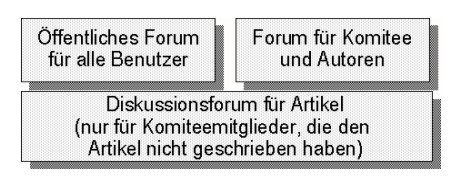
\includegraphics[width=10cm]{forum1}\end{center}
        \CoMa\ bietet verschiedene Foren f\"{u}r seine Benutzer an. Der Zugang zu diesen ist nur f\"{u}r bestimmte Rollen
            m\"{o}glich. (siehe Grafik)\\
            Zu den Artikeldiskussionen sind alle Benutzer zugelassen, die nicht Autor der Artikel sind, oder sich als
            Co-Autor markiert haben.

            Die Foren sind threadbasiert, wobei Threads von allen Forenbenutzern er\"{o}ffnet werden k\"{o}nnen. \CoMa\ kann
            Threads automatisch starten, wie zum Beispiel die Diskussionen zu nicht eindeutig bewerteten Artikeln.

            Bisher ist vorgesehen, dass die Foren nur mit den elementarsten Funktionen ausgestattet werden.

    \subsection{Verteilungsalgorithmus f\"{u}r die Artikel}
        \begin{center}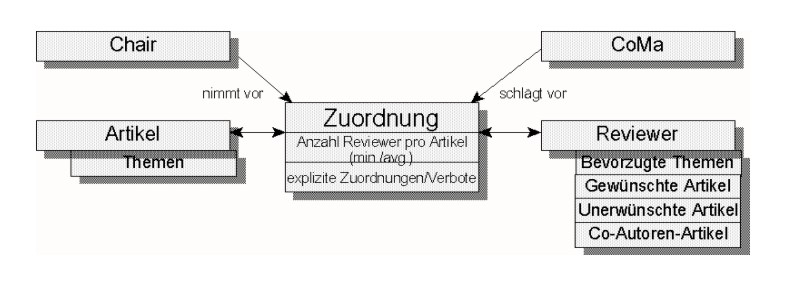
\includegraphics[width=17cm]{verteilung1}\end{center}
        \begin{description}
            \item[Eingabe:] \
            \begin{itemize}
                \item zu verteilende Artikel (mit deren Themeneinordnung)
                \item Reviewer (mit Auslastung, Pr\"{a}ferenz-/Ausschlussdaten)
                \item Vorgaben des Chairs (explizite Zuteilungen/Verbote)
            \end{itemize}
            \item[Konfigurationsdaten:] \
            \begin{itemize}
                \item minimale/durchschnittliche Anzahl von Reviewern pro Artikel
            \end{itemize}
            \item[Ausgabe:] \
            \begin{itemize}
                \item Verteilungsvorschlag
            \end{itemize}
            \item[Kriterien:] \
            \begin{itemize}
                \item Verbote werden eingehalten
                \item minimale Anzahl von Reviewern pro Artikel muss sichergestellt sein
                      (ggf. Meldung, wenn dieses nicht m\"{o}glich ist)
                \item m\"{o}glichst ausbalancierte Verteilung, so dass alle Reviewer etwa gleich viele Artikel zu bewerten haben
                \item m\"{o}glichst Ber\"{u}cksichtigung der Pr\"{a}ferenzen (Artikel, Themen)
            \end{itemize}
            \textbf{Bemerkung:} Die beiden letzten Kriterien sollten vom Algorithmus gewichtet ber\"{u}cksichtigt werden
            (z.B. im Verh\"{a}ltnis 3:2).
        \end{description}

    \subsection{Der Bewertungsvorgang im Detail}
        \begin{center}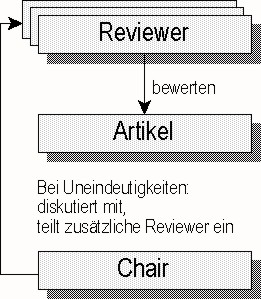
\includegraphics[width=6cm]{bewertung1}\end{center}
        Zum Ablauf des Bewertungsvorgangs siehe $\rightarrow$\ref{Reviewphase}.\\
        \\
        In unserem Konzept liegt der Schwerpunkt des Bewertungsvorgangs darauf, dass die ersten Artikelbewertungen
        \emph{ohne Fremdbeeinflussung} zustandekommen sollen. Aus diesem Grund werden f\"{u}r Reviewer die Bewertungen und Identit\"{a}ten
        ihrer Reviewergruppe sowie der Zugang zur Artikeldiskussion erst dann zug\"{a}nglich, sobald sie ihre erste Bewertung
        abgegeben haben. Ist es einem Reviewer nicht m\"{o}glich, ein erstes Urteil zu f\"{a}llen, kann er in einzelnen
        Kriterien zun\"{a}chst eine vorl\"{a}ufige Enthaltung abgeben.\\
        Im weiteren Verlauf kann jeder Reviewer seine Bewertung zu jedem Zeitpunkt revidieren.
        Ziel der Artikeldiskussion sollte es sein, dass alle Reviewer zu einer einheitlichen Artikelbewertung kommen.\\
        Der Chair kann zu jedem Zeitpunkt die Reviewphase f\"{u}r einen Artikel beenden und den Artikel als angenommen bzw.
        abgelehnt markieren.

\pagebreak
\section{Fazit: Begr\"{u}ndung und Diskussion der Ans\"{a}tze}
    \subsection{Was f\"{u}r Einschr\"{a}nkungen hat der Entwurf?}
    \begin{itemize}
        \item Die Arbeitsvorg\"{a}nge sind nur eingeschr\"{a}nkt automatisiert. So hilft \CoMa\ oft bei Entscheidungen,
            nimmt diese aber dem Benutzer nicht ab.

        \item Es gibt nur wenige (einstellbare) Parameter f\"{u}r die Algorithmen zur Artikelverteilung und -einsch\"{a}tzung.

        \item Es sind nur wenige Rollen in dem Modell verf\"{u}gbar, eventuell ist \emph{Accountsitting} erforderlich.
    \end{itemize}

    \subsection{Was zeichnet den Entwurf aus?}
    \begin{itemize}
        \item Der Entwurf von \CoMa\ ist leicht modularisierbar. (Rollenkonzept, Aktionenkonzept, erweiterte Features wie Teilnehmeranmeldung)

        \item \CoMa\ ist sehr flexibel, so ist es z.B. einfach Benutzer hinzuzuf\"{u}gen oder zu entfernen, die Phasen\"{u}berg\"{a}nge geschehen flie{\ss}end.

        \item \CoMa\ bietet einen Kommunikationsstandard f\"{u}r alle Benutzer an, da Nachrichten stets innerhalb des Systems versandt werden
              und Diskussion innerhalb des System \"{u}ber die Foren m\"{o}glich ist.

        \item Der Entwurf ist technisch unabh\"{a}ngig, nur eine Datenbank und ein Webfrontend werden ben\"{o}tigt.

        \item Als Webanwendung ist \CoMa\ portabel und f\"{u}r die Benutzer plattformunabh\"{a}ngig.

        \item \CoMa\ kann mehrere Konferenzen parallel verwalten.
    \end{itemize}


\end{document}
